%----------------------------------------------------------------------
\chapter{Implementation}
\label{chap:code-implementation}
%----------------------------------------------------------------------
\section{Software overview}
\label{sec:software-overview}
The code of the ODE solvers software is available on Github via this link: \href{https://github.com/FarmHJ/numerical-solver}{\underline{\emph{Github repository}}}. Software with version control can keep track of changes made to the code. It is very useful for large projects with collaborations. Aside from having version control, the software is fully documented. Details on its structure and functions are available at the link: \href{https://numerical-solver.readthedocs.io/en/latest/index.html}{\underline{\emph{software documentation}}}. Finally, the software is also full-tested to make sure the correctness of the code. More details of the testing infrastructure is described in later sections. 

To showcase the features of the code and to give a brief summary of the quality of the code, badges are displayed on the main page of the Github repository, as shown in Figure \ref{fig:badges}. The badges on this Github repository indicate that the code are tested to work on several python versions and operating systems. The badge `codecov' shows the code coverage of the software, which will also be described in details in the Section \ref{sec:testing}, together with the testing infrastructure. Finally, there is a status badge `Doctest' to verify that the documentation of the software is built successfully.

\begin{figure}
    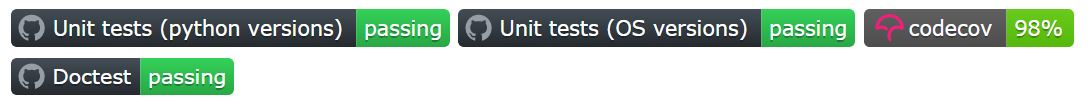
\includegraphics[width=0.95\columnwidth]{badges}
    \caption{Badges on Github repository.}
    \label{fig:badges}
\end{figure}

\section{Implemented numerical methods}
\label{sec:implemented-methods}
The numerical methods implemented in this software are classified into three classes: one-step methods, predictor-corrector methods and adaptive methods. The methods included are:
\begin{enumerate}
    \item One-step methods
    \begin{itemize}
        \item Euler's explicit method
        \item Euler's implicit method
        \item Trapezium rule method
        \item Four-stage Runge-Kutta method
    \end{itemize}
    \item Predictor-corrector method
    \begin{itemize}
        \item Euler-Trapezoidal method
    \end{itemize}
    \item Adaptive methods
    \begin{itemize}
        \item BS23 algorithm
        \item RKF45 algorithm
    \end{itemize}
\end{enumerate}

The main code on numerical methods are at \href{https://github.com/FarmHJ/numerical-solver/blob/main/solver/methods.py}{\underline{\emph{methods code}}}.

\section{Unit testing}
\label{sec:testing}
In the process of constructing the software, a unit testing infrastructure was put in place. The purpose of the unit testing is to create a robust and sustainable software. Written codes are tested to make sure it runs as intended and reproduces expected results. If code is tested while writing, it would be easier to fix bugs in the future. 

Code coverage is a measurement of the percentage of codes covered in the unit testing process. It is usually aim to achieve a 100\% code coverage. However, a 100\% code coverage does not necessarily mean that the code is correct or free of errors. Nevertheless, it provides some confidence that the code is implemented correctly.

Every method in this numerical-solver software is tested using the unittest Python library, a unit testing framework. The numerical solution produced by each method is tested to give the same solution as a manually calculated solution. The methods are mostly tested against the example model Eqs. \eqref{eqn:example_model}-\eqref{eqn:example-end}.

\section{Testing initialisation of problem}
\label{sec:test_init}
The initialisations of each class are tested to ensure that variables are initialised correctly and input type satisfies the requirements. For example, 

\begin{lstlisting}[language=Python, caption= {initialisation testing}, title={Testing initialisation of problem}, label={code:test_init}]
def test__init__(self):

    def func(x, y):
        return [-y[0]]
    x_min = 0
    x_max = 1
    initial_value = [1]
    mesh_points = 10

    problem = solver.OneStepMethods(
        func, x_min, x_max, initial_value, mesh_points)

    # Test initialisation
    self.assertEqual(problem.x_min, 0)
    self.assertEqual(problem.mesh_points, 10)

    # Test raised error for callable function
    with self.assertRaises(TypeError):
        solver.OneStepMethods(
            x_min, x_min, x_max, initial_value, mesh_points)

    # Test raised error if initial_value not list
    with self.assertRaises(TypeError):
        solver.OneStepMethods(
            func, x_min, x_max, 1, mesh_points)
\end{lstlisting}
A simple model with known solution is first initialised. Required inputs were checked to make sure the problem is set up properly, in line 14 and 15 of the code snippet above. To ensure that the inputs to the function are of the desired data type, errors are raised whenever the user inputs a wrong data type. The unit testing also tests that these errors are raised appropriately (line 17 to 25) whenever the data type does not satisfy the requirements. 

\section{Testing function}
\label{sec:test_func}
After making sure the problem is properly initialised, we then test that the numerical methods are working correctly. Take the adaptive method, BS23 algorithm, as an example, 
\begin{lstlisting}[language=Python, caption= {testing of function}, title={Testing execution of method}, label={code:test_func}]
def test_ode23(self):

    def func(x, y):
        return [-y[0]]
    x_min = 0
    x_max = 1
    initial_value = [1]
    
    problem = solver.AdaptiveMethod(
        func, x_min, x_max, initial_value, initial_mesh=0.5)
    mesh, soln = problem.ode23()
    
    # Test end point of mesh
    self.assertGreaterEqual(mesh[-1], 1.0)
    
    # Test mesh point
    self.assertAlmostEqual(mesh[1], 0.3483788976565)
    
    # Test solution at first stepsize
    self.assertAlmostEqual(soln[1][0], 0.7052580305097)
\end{lstlisting}
The method is first tested to execute computations up to the maximum mesh value indicated. Then, it is checked that the first adaptive mesh point and its solution, obtained from the software, matches the value computed manually. 

\section{Conclusion}
\label{sec:software-conclusion}
The software can solve any initial value problems with the general form \ref{eqn:initial_value} using the implemented numerical methods as listed in Section \ref{sec:implemented-methods}. The software can also handle initial value problems of higher dimension. Example of the use of the software can be found at the link: \href{https://nbviewer.jupyter.org/github/FarmHJ/numerical-solver/blob/main/examples/fitzhugh_nagumo.ipynb}{\underline{\emph{Example use of software}}}. All methods are tested, not only making sure all lines are tested, but also testing their functionalities. Moreover, the results from all notebooks (\ref{chap:link}) behaves as expected by theory. The time efficiency of the software is not a major concern of the project, thus some methods might take long periods of time to run.

The purpose of setting up a software with version control, documentation and testing is to create a robust and reusable software. These software engineering methods can give confidence in the correctness of the code and aid in the re-use of the code. By implementing these methods to this software, it will allow me to gain experience in developing the software engineering techniques that I will use throughout my D.Phil.
